\section{Викреслювання другого порядку}

Після того, як одним з методів було здійснено оптимізацію штрафної функції, 
виникає задача відновлення оптимальної розмітки --- треба знайти таку розмітку $k$
(або одну з таких розміток), якість якої дорівнює знайденій максимальній якості.
Для цього часто використовується алгоритм викреслювання другого порядку, також
відомий як алгоритм релаксації розмітки (relaxation labeling algorithm) \cite{savchynskyy,koval,rossi, Vodolazskii:2015}.

Структура графу аналогічна $(\max,+)$ задачі розмітки. Нехай $T$ --- скінченна
множина об'єктів, $K$ --- скінченна множина міток, $\Gamma \subset T^2$ --- множина сусідів, 
$N_t\subset T$ --- множина сусідів об'єкту $t\in T$.
Якості вершин та ребер --- бінарні значення,
 $q:T\times K\rightarrow\{0,1\}$ якості вершин, 
$g:\Gamma\times K^2\rightarrow\{0,1\}$ якості ребер. Вершина $(t,k), t\in T, k\in K$ вважається
допустимою, якщо відповідна їй якість $q_t(k)=1$. Аналогічним чином, ребро 
$((t,k),(t',k'))$, $t\in T$, $t'\in N_t$, $k\in K$, $k'\in K$ називається допустимим, якщо відповідна йому якість $g_{tt'}(k,k')=1$.

Допуcтимістю розмітки будемо називати
число $G\in\{0,1\}$
\begin{equation*}
      G=\bigvee_{k: T \rightarrow K} \bigwedge_{t\in T}q_t(k_t)\wedge\bigwedge_{tt' \in \Gamma} g_{tt'}(k,k').
  \end{equation*}
$(\bigvee, \bigwedge)$-задача полягає пошуку відповіді на питання ,,Чи існує 
така розмітка, для якої всі вершини та ребра є допустимими?'', тобто чи можна 
знайти таке значення $G$, що $G=1$.

\textbf{Правила викреслювання}

Вершина вважається допустимою, якщо відповідна їй якість $q_t(k)=1$, 
а також в неї входить принаймні одне допустиме ребро із кожного сусіднього
об'єкта $t'\in N_t$, тобто
\begin{equation*}
    q_t(k) = q_t(k)\wedge\bigwedge_{t'\in N_t}\bigvee_{k\in K}g_{tt'}(k,k'),
\end{equation*}
де $t\in T$, $k\in K$, $k'\in K$, $tt'\in\Gamma$.\\ 
Операція називається викреслюванням вершини.

Ребро вважається допустимим, якщо відповідна їй якість $g_{tt'}(k,k')=1$,
а також якщо вершини, які утворюють ребро $(t,k)$, $(t',k')$ є допустимими, тобто
\begin{equation*}
    g_{tt'}(k,k') = g_{tt'}(k,k')\wedge q_t(k)\wedge q_{t'}(k'),
\end{equation*}
де $t\in T, k\in K, k'\in K, tt'\in\Gamma$.\\
Операція називається викреслюванням ребра.

З наведеною постановкою задачі та описом основних операцій, наведемо повний 
алгоритм викреслювання другого порядку.

\begin{algorithm}[H]
    \caption{Алгоритм викреслювання другого порядку}
    \begin{algorithmic}
    \State \textbf{Вхід:} $(\bigvee, \bigwedge)$-задача розмітки
    \State \textbf{Вихід:} $G\in\{0,1\}$;
    \State \textbf{Ініціалізація}: 
    \begin{equation*}
    q^0=q, g^0=g, i=0.
    \end{equation*}
    \State \textbf{Крок 1}: 
    \begin{equation*}
        \begin{aligned}
        q^{i+1}_t(k) = q^i_t(k)\wedge\bigwedge_{t'\in N_t}\bigvee_{k\in K}g^i_{tt'}(k,k'),\\
        \forall t\in T, \forall k\in K.
    \end{aligned}
    \end{equation*}
    \State \textbf{Крок 2}: 
    \begin{equation*}
        \begin{aligned}
        g^{i+1}_{tt'}(k,k') = g^i_{tt'}(k,k')\wedge q^i_t(k)\wedge q^i_{t'}(k'),\\
        \forall t\in T, \forall t'\in N_t,  \forall k\in K, \forall k'\in K.
    \end{aligned}
    \end{equation*}
    \State \textbf{Крок 3}: 
    \begin{equation*}
        i = i+1.
    \end{equation*}

Якщо за ітерацію жодне значення з якостей $q, g$ не змінилося, повертаємося до кроку 1.
\State \textbf{Умова зупинки:}

Якщо на якомусь кроці $j>0$, виконуються умови
\begin{equation*}
    \begin{aligned}
    q^{j}_t(k) = 0, \\
    \forall t\in T, \forall k\in K,
\end{aligned}
\end{equation*}

\begin{equation*}
    \begin{aligned}
g^{j}_{tt'}(k,k') = 0, 
\forall t\in T, \forall t'\in N_t,  \forall k\in K, \forall k'\in K,
\end{aligned}
\end{equation*}
то це означає, що для задачі не існує такої розмітки, яка складається
з допустимих вершин та ребер, повертаємо $G=0$.

Якщо ж ні --- то це означає, що існує така розмітка, яка складається
з допустимих вершин та ребер, тоді повертаємо значення $G=1$.
\end{algorithmic}
\end{algorithm}


Алгоритм викреcлювання другого порядку полягає в багаторазовому застосуванні
операцій ,,викреслювання вершини'' та ,,викреcлювання ребра''. 

Алгоритм завершує роботу за скінченну кількість ітерацій, 
адже ніяка викреслена вершина або дужка не може
знову стати допустимою. Якщо після завершення роботи алгоритму деякі вершини
залишилися допустимими, то за певних умов \cite{savchynskyy} з множини допуcтимих вершин можна побудувати розмітку.

Загальна складність алгоритму викреcлювання другого порядку --- $\mathcal{O}(|T|^2\cdot |K|^2)$

\subsection{Застосування до $(\max,+)$ задачі розмітки}

Після оптимізації цільової функції двоїстої задачі шукають відповідь на запитання
чи існує допустима розмітка, і якщо існує, то як її знайти. Відповідь на перше
запитання дає алгоритм викреcлювання другого порядку. Для цього потрібно розглянути
наступне представлення задачі.

Маємо двоїсту $(\min, +)$ задачу розмітки на множині об'єктів $T$, множині 
міток $K$, та з репараметризованими якостями вершин 
$q^\varphi_t(k), t\in T, k\in K$ та репараметризованими якостями ребер
$g^\varphi_{tt'}(k,k')$, $tt'\in\Gamma$, $k\in K$, $k'\in K$.
За оригінальною постановкою задачі, ми хочемо мінімізувати значення
функції
\begin{equation*}
    \begin{aligned}
    E(\varphi) = \sum\limits_{tt'\in\Gamma}\max\limits_{k\in K, k'\in K}[ g_{tt'}(k,k')
    + \varphi_{tt'}(k) + \varphi_{t't}(k)] +\\
    \sum\limits_{t\in T}\max\limits_{k\in K}[ q_t(k) - \sum\limits_{t'\in N(t)} \varphi_{tt'}(k)] =
    \sum\limits_{tt'\in\Gamma}\max\limits_{k\in K, k'\in K}g^\varphi_{tt'}(k,k') + 
    \sum\limits_{t\in T}\max\limits_{k\in K}q^\varphi_t(k).
\end{aligned}
\end{equation*}

\begin{equation*}
    \varphi^* = \min_{\varphi} E(\varphi).
\end{equation*}
Нехай алгоритмом оптимізації ми знайшли підходяще або достатньо близьке
значення $\varphi^*$. Підставимо його у цільову функцію, і отримаємо
\begin{equation*}
    \begin{aligned}
    E(\varphi^*) =
    \sum\limits_{tt'\in\Gamma}\max\limits_{k\in K, k'\in K}g^{\varphi^*}_{tt'}(k,k') + 
    \sum\limits_{t\in T}\max\limits_{k\in K}q^{\varphi^*}_t(k).
\end{aligned}
\end{equation*}
З цієї рівності чітко видно, що шукана розмітка --- це та, для якої ми обираємо мітку з
максимальною якістю для кожного об'єкту, і одночасно з цим, вибираємо такі ребра, які мають
максимальну вагу. Якщо алгоритм оптимізації не досяг глобального оптимуму, то 
можуть виникнути проблеми. Розмітка --- це не просто вибір мітки в кожному об'єкті, 
крім того, потрібно також щоб обрані мітки були з'єднані ребром. 

Припустимо, що
для якогось об'єкту $t\in T$ ми обрали мітку з максимальною якістю $k_t^*\in K$.
Для сусіднього об'єкту $t'\in N_t$ обрали мітку $k_{t'}^*\in K$. Тепер потрібно 
обрати найкраще ребро для пари $tt'\in\Gamma$. Нехай ребро з найкращою якістю
буде $((t,l),(t',l'))$, $t\in T$, $t'\in T$, $l\in K$, $l'\in K$. Проблемою в даному випадку
буде те, що з обраного набору міток не можливо обрати розмітку (для пари об'єктів).
Якщо така ситуація сталася при хоча б для однієї пари об'єктів $tt'\in\Gamma$, то 
отримати розмітку вже неможливо. Можливі також схожі випадки, наприклад 
$k_{t'}^*=l, k_{t'}^*\neq l'$, тобто ребро входить не в мітку з максимальною
вагою, і т.д. На рис. \ref{fig:graph_example_cross} зображено приклад особливого випадку, який
вимагає додаткової уваги.
\begin{figure}[h]
    \centering
    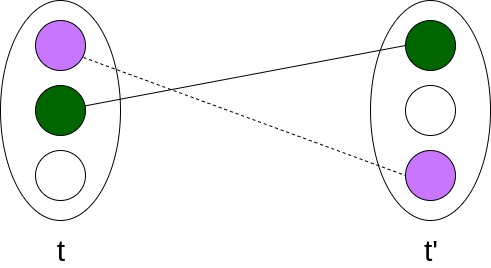
\includegraphics[width=0.5\textwidth]{images/multiple_choice.jpg}
    \caption{Приклад випадку, коли неможливо обрати розмітку. Фіолетовим кольором
    позначені вершини з максимальною якістю $q$, зеленим кольором позначені вершини, які
    утворюють ребро з максимальною якістю $g$. Лініями позначені можливі ребра,
    які поєднують ,,кращі'' вершини.}
    \label{fig:graph_example_cross}
  \end{figure}

Для приблизного розв'язку іноді опускають ці неточності, та обирають мітку в об'єкті 
шляхом вибору ребра із максимальною якістю. Часто такий підхід дає прийнятні результати 
на практиці, хоча йому й бракує теоретичного підґрунтя. 

Для уникнення таких випадків, ми маємо задачу, після того, як здійснили оптимізацію.
Сформулюємо $(\bigvee, \bigwedge)$-задачу розмітки.

Множина об'єктів $T$ та множина міток $K$, структура сусідства $\Gamma$ задачі будуть такими ж, як і для 
$(\max,+)$ задачі. Нові якості задачі будуть задаватися наступними функціями
\begin{equation*}
    \begin{cases}
    \label{eqn:strict_optimal}
    q_t(k) = \llbracket q^{\varphi}_t(k) = \max\limits_{l\in K}q^{\varphi}_t(l) \rrbracket, & t\in T, k\in K,\\
    g_{tt'}(k,k') = \llbracket g^\varphi_{tt'}(k,k')=\max\limits_{l\in K, l'\in K}g^{\varphi}_{tt'}(l,l')\rrbracket,
     & tt'\in\Gamma, k\in K, k'\in K.
\end{cases}
\end{equation*}
При такій постановці ми якраз і будемо перевіряти, чи можливо обрати найкращі
мітки у вершинах та ребрах таким чином, щоб з них можна було скласти розмітку.
Варто відмітити, що виконання умов (\ref{eqn:strict_optimal}) можливе лише за
умови, що функція $P(\varphi)$ --- досягає глобального оптимуму в точці $\varphi^*$.  

Іноді алгоритми оптимізації гарантовано сходяться до глобального оптимуму
тільки при нескінченній кількості кроків, що неможливо для практичного застосування.
Через це часто вводяться послаблені умови допустимості вершин та ребер.
\begin{equation*}
    \begin{cases}
    \label{eqn:epsilon_optimal}
    q_t(k) = \llbracket |q^{\varphi}_t(k) - \max\limits_{l\in K}q^{\varphi}_t(l)|\leq \varepsilon\rrbracket, & t\in T, k\in K,\\
    g_{tt'}(k,k') = \llbracket|g^\varphi_{tt'}(k,k')-\max\limits_{l\in K, l'\in K}g^{\varphi}_{tt'}(l,l')|\leq\varepsilon\rrbracket,
     & tt'\in\Gamma, k\in K, k'\in K,\\
    \varepsilon \in \mathbb{R_+}.
\end{cases}
\end{equation*}
Фактично вирішується оптимізаційна задача виду
\begin{equation*}
    k^*(\varepsilon)\in\arg\bigvee_{k:T\rightarrow K}\bigwedge_{tt'\in\Gamma}
    \llbracket|g^\varphi_{tt'}(k,k')-\max\limits_{l\in K, l'\in K}g^{\varphi}_{tt'}(l,l')|\leq\varepsilon\rrbracket\wedge
    \bigwedge_{t\in T}\llbracket|q^{\varphi}_t(k) - \max\limits_{l\in K}q^{\varphi}_t(l)|\leq \varepsilon\rrbracket.
\end{equation*}

Отримана розмітка називається $\varepsilon$-допустимою. Варто відмітити, що
при такому послаблені, ми можемо й не досягти оптимального значення після оптимізації,
(хоча й будемо $\varepsilon$-близькі до нього). 
Знайдена розмітка при умові $\varepsilon\rightarrow 0$ буде наближатися до оптимальної.
Такі умови дозволяють точно вирішувати ширший клас задач за скінченний час, а також
контролювати відхилення знайденого оптимуму від глобального, більше того, відхилення від $\varepsilon$
слугує метрикою, з допомогою якої ми можемо балансувати швидкість розв'язку та точність вирішення.


Для нових якостей вершин $q_t(k)$, $t\in T$, $k\in K$ та якостей ребер
$g_{tt'}(k,k')$, $tt'\in\Gamma$, $k\in K$, $k'\in K$ розв'яжемо 
$(\bigvee, \bigwedge)$-задачу розмітки. Якщо отримали $G=0$, то це означає, 
що для даної знайденої репараметризації $\varphi$ не існує допустимої розмітки, тобто
принаймні для однієї пари об'єктів обрані кращі мітки для вершин не стикуються з обраними
кращими мітками для ребер. Якщо ж $G=1$, то це означає, що існує розмітка, для 
яка складається із допустимих вершин та ребер, які стикуються між собою. 

Невикреслена множина 
вершин та ребер називається $\varepsilon$-узгодженим набором вершин та ребер.
Якщо алгоритм завершив свою роботу із відповіддю $G=0$,
то $\varepsilon$-узгоджений набір вершин та ребер буде порожньою множиною.

Хоча алгоритм викреслювання другого порядку і дозволяє перевіряти наявність
потрібної розмітки, алгоритм не дає змоги відшукати її.